%TODO: while Loop 
%TODO: for Loop 
%TODO: break and continue 
%TODO: Pass 
%TODO:Common errors in loops 

% \begin{frame}[fragile]{Loops}
%     \tit{While loops}
%  \begin{itemize}[<+->]
%     \item A \texttt{while} loop allows a block of instructions to execute as long as (or while) a condition is \texttt{True}.
%     \item When the condition is \texttt{False}, the loop's body is ignored, and the execution continues at the first statement after the body of the \texttt{while} loop.
%     \item The body of the while loop is determined through indentation.
%     \item If the condition always evaluates to \texttt{True}, the body will be executed infinitely, that's what we call {\bf infinite loop problem}.
%     \item We must update the condition's variables to avoid the infinite loop.
%     \item Generally, we use while loops when we don't know the number of executions of the loop's body.
% \end{itemize}
% \end{frame}
% \begin{frame}[fragile]{Loops}
% \tit{\texttt{while} syntax and flowchart}
%     \texttt{while}'s loop syntax is:



% \begin{lstlisting}[showstringspaces=false,language=python, caption={while syntax}]
% while (condition):
%     block_instructions #body
% \end{lstlisting}            
% \begin{figure}
%         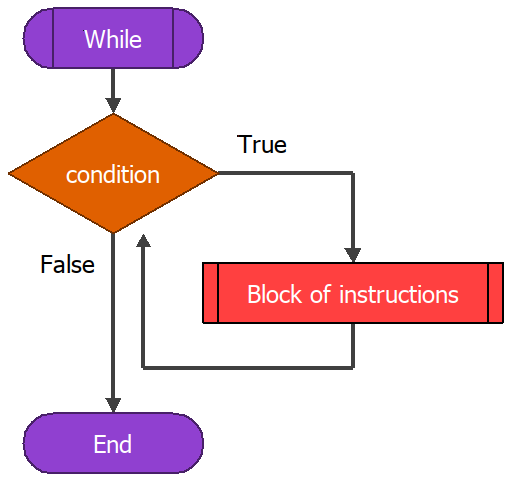
\includegraphics[scale=.24]{img/While_Chart.png}
% \caption{while flowchart}
%     \end{figure}
% \end{frame}
% \begin{frame}[fragile]{Loops}
%     \tit{While loop with else}
%     \texttt{while} loop can have an optional \text{else}. The \text{else} body is executed if the condition is \texttt{False} 
% \begin{lstlisting}[numbers=left,showstringspaces=false,language=python]
% counter = 0
% while counter < 3:
%     print("Inside while body")
%     counter = counter + 1
% else:
%     print("Inside else body")
% \end{lstlisting}        
% \end{frame}
% \begin{frame}[fragile]{Loops}
%     \tit{\texttt{for} loops}
%     \begin{itemize}
%         \item The \texttt{for} loop allows to execute a block of instructions multiple times. In fact, this loop is used to iterate over iterable objects.
%         \item An {\bf iterable objects} is a sequence of items capable of returning its members one by one, for example \texttt{list} and \texttt{strings} are iterable objects.
%     \end{itemize}
%     The \texttt{for} loop  syntax in python is:
% \begin{lstlisting}[showstringspaces=false,language=python]
% for loop_var in iterable_object:
%     for_block #body
% \end{lstlisting}   
% The variable \texttt{loop\_var} take the values of the items of the iterable object. Loop continues until the variable reach the last item in the sequence.


% The body of the loop must be indented.
% % TODO: range() function
% \end{frame}
% \begin{frame}[fragile]{Loops}
%     \exercise{Draw the flowchart of for loop}
% % \begin{figure}
% %         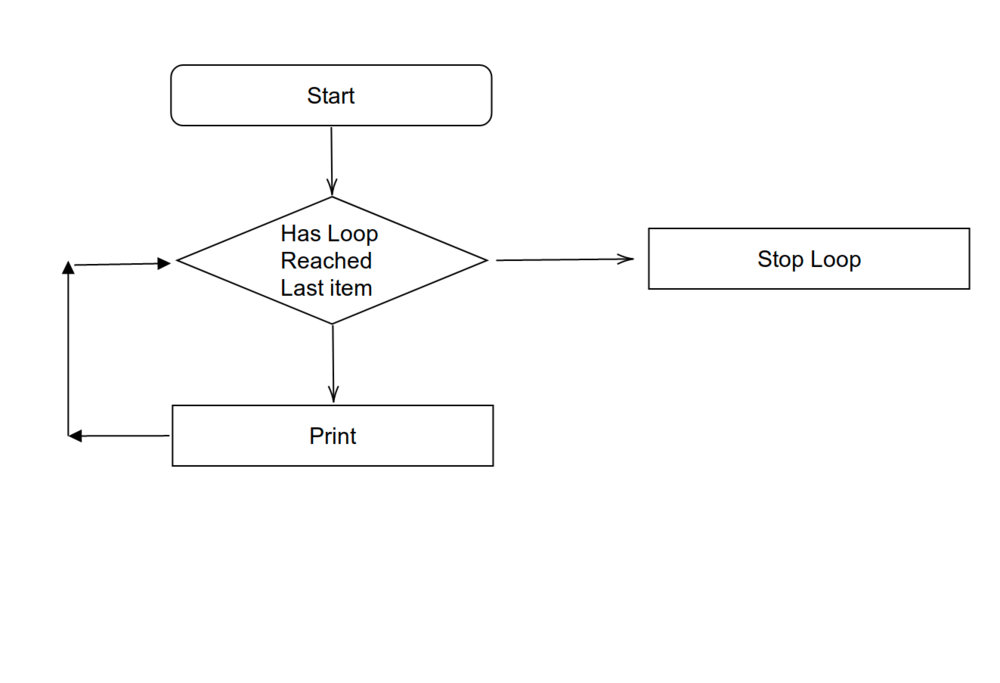
\includegraphics[scale=.24]{img/For_Chart.png}
% % \caption{for flowchart}
% %     \end{figure}
% \tit{Example: Python \texttt{for} Loop}
% \begin{lstlisting}[numbers=left,showstringspaces=false,language=python]
% word="NHSM"
% for letter in word:
%     print(letter)
% \end{lstlisting}        
% \end{frame}
\begin{frame}[fragile]{Loops}
    \tit{\texttt{range()} function}
    In python, we can use the {range()} function to generate a sequence of numbers.
    \pause
    The usage of range function is as follows:
        $$\texttt{range([start], stop,[step\_size])}$$
\begin{align*}
    \texttt{start}: &\text{(Optional). An integer number specifying at which position to start.}\\ 
                    &\text{Default is 0.}\\
    \texttt{stop}:&\text{An integer number specifying at which position to stop}\\
                  & \text{(not included).}\\
    \texttt{step}:&\text{(Optional). An integer number specifying the incrementation.}\\
                  &\text{Default is 0.}
\end{align*}
\pause
    Try this
    \begin{lstlisting}[numbers=left,showstringspaces=false,language=python]
print(range(10))
print(list(range(10)))
print(list(range(2, 8)))
print(list(range(2, 20, 3)))
    \end{lstlisting}        
\end{frame}
\begin{frame}[fragile]{Loops}
    \tit{Examples}

    \begin{lstlisting}[numbers=left,showstringspaces=false,language=python]
        #example1
        for i in range(9):
            print(i)
        else:
            print("No items left.")
        #example2 (else)
        digits=[6,2,9]
        for digit in digits:
            print(digit)
        else:
            print("No items left.")
        #example3
        # Program to iterate through a list using indexing
        names = ['Omar', 'Mohamed', 'Ali']
        # iterate over the list using index
        for i in range(len(names)):
            print("His name is", names[i])
    \end{lstlisting}
\end{frame}
\begin{frame}[fragile]{Loops}
    \tit{\texttt{break} and \texttt{continue} }
    \begin{itemize}[<+->]
        \item The \texttt{break} statement terminates the loop containing it. The program execute the statement immediately after the body of the loop.
        \item The \texttt{continue} statement is used to skip the rest of the code inside a loop for the current iteration only. Loop does not terminate but continues on with the next iteration.
    \end{itemize}
\onslide<1->\begin{lstlisting}[numbers=left,showstringspaces=false,language=python]
name="NHSM"
for letter in name:
    if (letter=='S'):
        break
    print(letter)
\end{lstlisting}
\onslide<2>
\begin{lstlisting}[numbers=left,showstringspaces=false,language=python]
    name="NHSM"
    for letter in name:
        if (letter=='S'):
            continue
        print(letter)
    \end{lstlisting}
\end{frame}
% \begin{frame}[fragile]{Loops}
%     \tit{}
%     \begin{lstlisting}[numbers=left,showstringspaces=false,language=python]
%     \end{lstlisting}        
% \end{frame}
% \begin{frame}[fragile]{Loops}
%     \tit{}
%     \begin{lstlisting}[numbers=left,showstringspaces=false,language=python]
%     \end{lstlisting}        
% \end{frame}
% \begin{frame}[fragile]{Loops}
%     \tit{}
%     \begin{lstlisting}[numbers=left,showstringspaces=false,language=python]
%     \end{lstlisting}        
% \end{frame}
% \begin{frame}[fragile]{Loops}
%     \tit{}
%     \begin{lstlisting}[numbers=left,showstringspaces=false,language=python]
%     \end{lstlisting}        
% \end{frame}
% \begin{frame}[fragile]{Loops}
%     \tit{}
%     \begin{lstlisting}[numbers=left,showstringspaces=false,language=python]
%     \end{lstlisting}        
% \end{frame}